\section{Contruction}
The phototransistor is just an ordinary BJT transistor with the base terminal exposed for illumination.
It can be found of both PNP and NPN types. It has more base and collector regions than a conventioncal BJT \cite{phteff}.

Mechanical issues of placement of the phototransistor or photodiode are dictated by the application, modes of use, user interaction, and many other factors which must be carefully considered in the product design. Consistency of this optical path is critical.
Even minute variations due to manufacturing tolerances, board flexing, dust, and other expected and/or somewhat abnormal use must be considered.
Mechanical issues of placement of the phototransistor or photodiode are dictated by the application, modes of use, user interaction, and many other factors which must be carefully considered in the product design.
Consistency of this optical path is critical.
Even minute variations due to manufacturing tolerances, board flexing, dust, and other expected and/or somewhat abnormal use must be considered. \cite{phteff}

\begin{figure}[H]
    \centering
    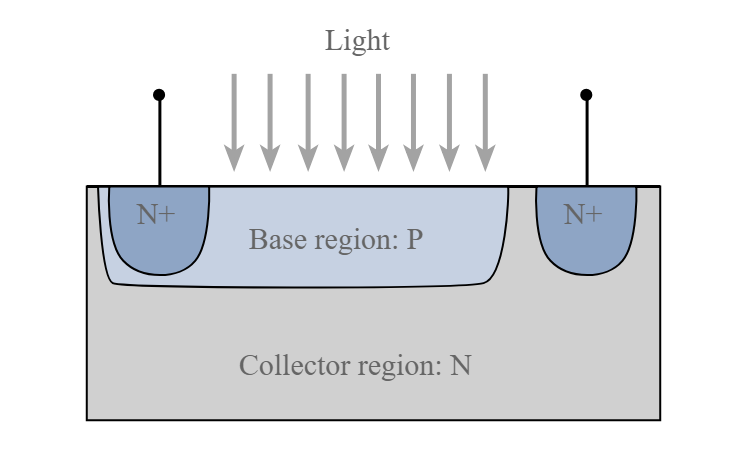
\includegraphics[width=0.75\textwidth]{phototransistor-construction.png}
    \caption{Construction of an NPN Phototransistor}
    \label{fig:phototransitor-construction}
\end{figure}

Fig.  \ref{fig:phototransitor-construction} shows the construction of a phototransistor of NPN type.
When compared to normal transistor, in photo transistor the base and collector area is large.
The base area is increased to increase the amount of current generated. Because more the light falls more the current is generated.
Earlier it was made up of single semiconductor material like silicon or germanium.
Recently photo transistors are made up of Gallium and Arsenic to obtain higher efficiency.
Finally photo transistor is placed inside a metallic case and a lens is kept at the top of the case to absorb the incident radiation. \cite{phototransistorconstruction}

\section{Circuit Diagram}
\begin{figure}[H]
    \centering
    \begin{circuitikz}[american] 
    \draw
    (0,0) node[npn, photo] (ps){};
    \node[anchor=west, font=\footnotesize] at (ps.collector) {\textit{C}};
    \node[anchor=north, font=\footnotesize] at (ps.base) {\textit{B}};
    \node[anchor=west, font=\footnotesize] at (ps.emitter) {\textit{E}};
    \end{circuitikz}
    \caption{NPN Phototransistor}
    \label{fig:symbol}
\end{figure}

\noindent Fig. \ref{fig:symbol} is the symbol for an npn phototransistor. Here the \(B\) represents the base terminal,
\(C\) represents the collector terminal and \(E\) represents the emitter terminal. The base terminal is exposed to light and that generates current.


\begin{figure}[H]
\centering
\begin{circuitikz}[american]
    \node[npn, photo] at (0,0) (npn) {};
    \draw (npn.C) to[short] (0,1.5) node[vcc, anchor=south] (vcc) {$V_{CC}$};
    \draw (npn.E) to[short] (0,-1) node[anchor=east] (vout) {}
    to[R, l=$R1$] (0,-4) node[ground] () {} node[anchor=west] () {GND};
    \draw (vout) to[short, -o] ++(1.5,0) node[anchor=west] () {$V_{out}$};
\end{circuitikz}
\caption{A Simple Light Detector Circuit}
\label{fig:lightdetector}
\end{figure}

\noindent Fig. \ref{fig:lightdetector} shows a very simple light detector circuit.
When there is no light, $V_{out}$ remains very close to zero (there is a small amount of voltage present due to dark current).
When light falls on the phototransistor, $V_{out}$ rises and has some positive voltage. This voltage can be picked up and used in microcontrollers.